\begin{frame}{\problemtitle}
	\begin{block}{Problem}
		Given an array $t_1, \ldots, t_n$, sort it by applying the minimum number of permutations
		which have only one cycle of length $> 1$. 
	\end{block}
	\pause
	\begin{block}{Solution}
		\begin{itemize}
			\item Already sorted? $\rightarrow$ answer $0$
			\pause
			\item Check if one operation is sufficient:
			\begin{itemize}
				\item Let $s$ be the sorted version of $t$.
				\item Build the graph $G$ with directed edges $s_i \rightarrow t_i$.
				\pause
				\item $G$ has multiple components (with $>0$ edges)? $\rightarrow$ one operation is not sufficient.
				\item Otherwise $\rightarrow$ one operation suffices, construct Euler cycle 
			\end{itemize}
			\pause
			\item Two operations are always sufficient!
		\end{itemize}
	\end{block}
\end{frame}

\begin{frame}{\problemtitle}
	\begin{block}{Lemma}
		Every permutation is the composition of two cycles.
	\end{block}
	\begin{block}{Proof by picture}
		\centering
		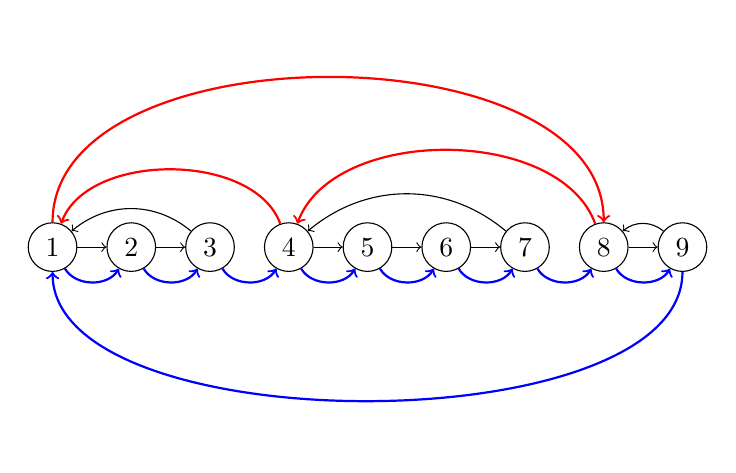
\begin{tikzpicture}
			\node[draw=black,shape=circle] (1) at (0, 0) {1};
			\node[draw=black,shape=circle] (2) at (1, 0) {2};
			\node[draw=black,shape=circle] (3) at (2, 0) {3};
			\node[draw=black,shape=circle] (4) at (3, 0) {4};
			\node[draw=black,shape=circle] (5) at (4, 0) {5};
			\node[draw=black,shape=circle] (6) at (5, 0) {6};
			\node[draw=black,shape=circle] (7) at (6, 0) {7};
			\node[draw=black,shape=circle] (8) at (7, 0) {8};
			\node[draw=black,shape=circle] (9) at (8, 0) {9};

			\draw[->] (1) -- (2);
			\draw[->] (2) -- (3);
			\draw[->] (3) to[out=140,in=40] (1);
			\draw[->] (4) -- (5);
			\draw[->] (5) -- (6);
			\draw[->] (6) -- (7);
			\draw[->] (7) to[out=140,in=40] (4);
			\draw[->] (8) -- (9);
			\draw[->] (9) to[out=140,in=40] (8);

			\onslide<2->{
				\draw[->,draw=blue,thick] (1) to[out=300,in=240] (2);
				\draw[->,draw=blue,thick] (2) to[out=300,in=240] (3);
				\draw[->,draw=blue,thick] (3) to[out=300,in=240] (4);
				\draw[->,draw=blue,thick] (4) to[out=300,in=240] (5);
				\draw[->,draw=blue,thick] (5) to[out=300,in=240] (6);
				\draw[->,draw=blue,thick] (6) to[out=300,in=240] (7);
				\draw[->,draw=blue,thick] (7) to[out=300,in=240] (8);
				\draw[->,draw=blue,thick] (8) to[out=300,in=240] (9);
				\draw[->,draw=blue,thick] (9) to[out=270,in=270, looseness=0.7] (1);
			}

			\onslide<3->{
				\draw[->,draw=red,thick] (1) to[out=90,in=90,looseness=0.9] (8);
				\draw[->,draw=red,thick] (8) to[out=110,in=70,looseness=0.9] (4);
				\draw[->,draw=red,thick] (4) to[out=110,in=70,looseness=0.9] (1);
			}

		\end{tikzpicture}
	\end{block}
\end{frame}
